\titre{31}
\theme{trigo}
\auteur{Nathan Scheinmann}
\niveau{1M}
\source{sesamath-1M-trigo}
\type{serie}
\piments{2}
\pts{}
\annee{2425}

\contenu{
	\tcblower
	Soit un cercle de centre $C$ et de rayon $6~\text{cm}$. De $A$, un point extérieur au cercle, part une demi-droite $d_{AF}$ issue de $A$ et tangente au cercle au point $D$.
	On a un triangle $\triangle CAD$, un triangle $\triangle CAE$ avec $CE$ perpendiculare à $CA$, et un triangle $\triangle AGF$ avec $G$ un point commun à $CA$ et à la tangente $GF$. 

	\begin{center}
		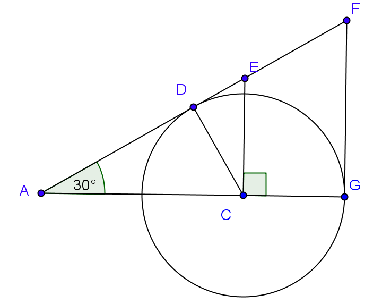
\includegraphics[scale=1]{../medias/1M/trigo/1M-exo-31}
	\end{center}

	Calculer les longueurs des trois côtés de ces trois triangles. 
}
\correction{

}

